% Options for packages loaded elsewhere
\PassOptionsToPackage{unicode}{hyperref}
\PassOptionsToPackage{hyphens}{url}
%
\documentclass[
]{article}
\usepackage{amsmath,amssymb}
\usepackage{lmodern}
\usepackage{iftex}
\ifPDFTeX
  \usepackage[T1]{fontenc}
  \usepackage[utf8]{inputenc}
  \usepackage{textcomp} % provide euro and other symbols
\else % if luatex or xetex
  \usepackage{unicode-math}
  \defaultfontfeatures{Scale=MatchLowercase}
  \defaultfontfeatures[\rmfamily]{Ligatures=TeX,Scale=1}
\fi
% Use upquote if available, for straight quotes in verbatim environments
\IfFileExists{upquote.sty}{\usepackage{upquote}}{}
\IfFileExists{microtype.sty}{% use microtype if available
  \usepackage[]{microtype}
  \UseMicrotypeSet[protrusion]{basicmath} % disable protrusion for tt fonts
}{}
\makeatletter
\@ifundefined{KOMAClassName}{% if non-KOMA class
  \IfFileExists{parskip.sty}{%
    \usepackage{parskip}
  }{% else
    \setlength{\parindent}{0pt}
    \setlength{\parskip}{6pt plus 2pt minus 1pt}}
}{% if KOMA class
  \KOMAoptions{parskip=half}}
\makeatother
\usepackage{xcolor}
\IfFileExists{xurl.sty}{\usepackage{xurl}}{} % add URL line breaks if available
\IfFileExists{bookmark.sty}{\usepackage{bookmark}}{\usepackage{hyperref}}
\hypersetup{
  pdftitle={01\_cleanOccurrences},
  pdfauthor={Daniela Linero},
  hidelinks,
  pdfcreator={LaTeX via pandoc}}
\urlstyle{same} % disable monospaced font for URLs
\usepackage[margin=1in]{geometry}
\usepackage{color}
\usepackage{fancyvrb}
\newcommand{\VerbBar}{|}
\newcommand{\VERB}{\Verb[commandchars=\\\{\}]}
\DefineVerbatimEnvironment{Highlighting}{Verbatim}{commandchars=\\\{\}}
% Add ',fontsize=\small' for more characters per line
\usepackage{framed}
\definecolor{shadecolor}{RGB}{248,248,248}
\newenvironment{Shaded}{\begin{snugshade}}{\end{snugshade}}
\newcommand{\AlertTok}[1]{\textcolor[rgb]{0.94,0.16,0.16}{#1}}
\newcommand{\AnnotationTok}[1]{\textcolor[rgb]{0.56,0.35,0.01}{\textbf{\textit{#1}}}}
\newcommand{\AttributeTok}[1]{\textcolor[rgb]{0.77,0.63,0.00}{#1}}
\newcommand{\BaseNTok}[1]{\textcolor[rgb]{0.00,0.00,0.81}{#1}}
\newcommand{\BuiltInTok}[1]{#1}
\newcommand{\CharTok}[1]{\textcolor[rgb]{0.31,0.60,0.02}{#1}}
\newcommand{\CommentTok}[1]{\textcolor[rgb]{0.56,0.35,0.01}{\textit{#1}}}
\newcommand{\CommentVarTok}[1]{\textcolor[rgb]{0.56,0.35,0.01}{\textbf{\textit{#1}}}}
\newcommand{\ConstantTok}[1]{\textcolor[rgb]{0.00,0.00,0.00}{#1}}
\newcommand{\ControlFlowTok}[1]{\textcolor[rgb]{0.13,0.29,0.53}{\textbf{#1}}}
\newcommand{\DataTypeTok}[1]{\textcolor[rgb]{0.13,0.29,0.53}{#1}}
\newcommand{\DecValTok}[1]{\textcolor[rgb]{0.00,0.00,0.81}{#1}}
\newcommand{\DocumentationTok}[1]{\textcolor[rgb]{0.56,0.35,0.01}{\textbf{\textit{#1}}}}
\newcommand{\ErrorTok}[1]{\textcolor[rgb]{0.64,0.00,0.00}{\textbf{#1}}}
\newcommand{\ExtensionTok}[1]{#1}
\newcommand{\FloatTok}[1]{\textcolor[rgb]{0.00,0.00,0.81}{#1}}
\newcommand{\FunctionTok}[1]{\textcolor[rgb]{0.00,0.00,0.00}{#1}}
\newcommand{\ImportTok}[1]{#1}
\newcommand{\InformationTok}[1]{\textcolor[rgb]{0.56,0.35,0.01}{\textbf{\textit{#1}}}}
\newcommand{\KeywordTok}[1]{\textcolor[rgb]{0.13,0.29,0.53}{\textbf{#1}}}
\newcommand{\NormalTok}[1]{#1}
\newcommand{\OperatorTok}[1]{\textcolor[rgb]{0.81,0.36,0.00}{\textbf{#1}}}
\newcommand{\OtherTok}[1]{\textcolor[rgb]{0.56,0.35,0.01}{#1}}
\newcommand{\PreprocessorTok}[1]{\textcolor[rgb]{0.56,0.35,0.01}{\textit{#1}}}
\newcommand{\RegionMarkerTok}[1]{#1}
\newcommand{\SpecialCharTok}[1]{\textcolor[rgb]{0.00,0.00,0.00}{#1}}
\newcommand{\SpecialStringTok}[1]{\textcolor[rgb]{0.31,0.60,0.02}{#1}}
\newcommand{\StringTok}[1]{\textcolor[rgb]{0.31,0.60,0.02}{#1}}
\newcommand{\VariableTok}[1]{\textcolor[rgb]{0.00,0.00,0.00}{#1}}
\newcommand{\VerbatimStringTok}[1]{\textcolor[rgb]{0.31,0.60,0.02}{#1}}
\newcommand{\WarningTok}[1]{\textcolor[rgb]{0.56,0.35,0.01}{\textbf{\textit{#1}}}}
\usepackage{graphicx}
\makeatletter
\def\maxwidth{\ifdim\Gin@nat@width>\linewidth\linewidth\else\Gin@nat@width\fi}
\def\maxheight{\ifdim\Gin@nat@height>\textheight\textheight\else\Gin@nat@height\fi}
\makeatother
% Scale images if necessary, so that they will not overflow the page
% margins by default, and it is still possible to overwrite the defaults
% using explicit options in \includegraphics[width, height, ...]{}
\setkeys{Gin}{width=\maxwidth,height=\maxheight,keepaspectratio}
% Set default figure placement to htbp
\makeatletter
\def\fps@figure{htbp}
\makeatother
\setlength{\emergencystretch}{3em} % prevent overfull lines
\providecommand{\tightlist}{%
  \setlength{\itemsep}{0pt}\setlength{\parskip}{0pt}}
\setcounter{secnumdepth}{-\maxdimen} % remove section numbering
\ifLuaTeX
  \usepackage{selnolig}  % disable illegal ligatures
\fi

\title{01\_cleanOccurrences}
\author{Daniela Linero}
\date{9/7/2021}

\begin{document}
\maketitle

\begin{Shaded}
\begin{Highlighting}[]
\CommentTok{\# Load libraries}
\FunctionTok{library}\NormalTok{(tidyverse) }\CommentTok{\# For data wrangling}
\FunctionTok{library}\NormalTok{(data.table) }\CommentTok{\# To load multiple files at once}
\FunctionTok{library}\NormalTok{(Hmisc) }\CommentTok{\# For the \%nin\% operator }
\FunctionTok{library}\NormalTok{(CoordinateCleaner) }\CommentTok{\# To flag records with erroneous coordinates}
\FunctionTok{library}\NormalTok{(countrycode) }\CommentTok{\# Associated with coordinate cleaner}
\FunctionTok{library}\NormalTok{(rgdal) }\CommentTok{\# To handle vector data }
\FunctionTok{library}\NormalTok{(sp) }\CommentTok{\# To handle vector data }
\FunctionTok{library}\NormalTok{(knitr) }\CommentTok{\# For markdown files}
\end{Highlighting}
\end{Shaded}

\hypertarget{load-ocurrences-of-all-species-from-ebird}{%
\subsubsection{1. Load ocurrences of all species from
ebird}\label{load-ocurrences-of-all-species-from-ebird}}

\begin{Shaded}
\begin{Highlighting}[]
\NormalTok{data }\OtherTok{\textless{}{-}} 
  \FunctionTok{list.files}\NormalTok{(}\AttributeTok{pattern =} \StringTok{"*.txt"}\NormalTok{) }\SpecialCharTok{\%\textgreater{}\%} 
  \FunctionTok{map\_df}\NormalTok{(}\SpecialCharTok{\textasciitilde{}}\FunctionTok{fread}\NormalTok{(., }\AttributeTok{encoding =} \StringTok{\textquotesingle{}UTF{-}8\textquotesingle{}}\NormalTok{))}
\end{Highlighting}
\end{Shaded}

\hypertarget{remove-some-species-that-had-wrong-information-about-home-ranges}{%
\subsubsection{2. Remove some species that had wrong information about
home
ranges}\label{remove-some-species-that-had-wrong-information-about-home-ranges}}

\begin{Shaded}
\begin{Highlighting}[]
\NormalTok{data }\OtherTok{\textless{}{-}}\NormalTok{ data }\SpecialCharTok{\%\textgreater{}\%} 
  \FunctionTok{filter}\NormalTok{(}\StringTok{\textasciigrave{}}\AttributeTok{SCIENTIFIC NAME}\StringTok{\textasciigrave{}} \SpecialCharTok{\%nin\%} \FunctionTok{c}\NormalTok{(}\StringTok{"Campylorhynchus nuchalis"}\NormalTok{, }\StringTok{"Chlorochrysa phoenicotis"}\NormalTok{)) }\SpecialCharTok{\%\textgreater{}\%} \FunctionTok{droplevels}\NormalTok{()}
\end{Highlighting}
\end{Shaded}

\hypertarget{delete-records-with-certain-protocols}{%
\subsubsection{3. Delete records with certain
protocols}\label{delete-records-with-certain-protocols}}

\begin{Shaded}
\begin{Highlighting}[]
\CommentTok{\# Select travelling, stationary and area protocols  }
\NormalTok{data }\OtherTok{\textless{}{-}}\NormalTok{ data }\SpecialCharTok{\%\textgreater{}\%} 
  \FunctionTok{filter}\NormalTok{(}\StringTok{\textasciigrave{}}\AttributeTok{PROTOCOL TYPE}\StringTok{\textasciigrave{}} \SpecialCharTok{\%in\%} \FunctionTok{c}\NormalTok{(}\StringTok{"Traveling"}\NormalTok{, }\StringTok{"Stationary"}\NormalTok{, }\StringTok{"Area"}\NormalTok{)) }\SpecialCharTok{\%\textgreater{}\%} 
  \FunctionTok{droplevels}\NormalTok{()}
\end{Highlighting}
\end{Shaded}

\hypertarget{delete-records-with-routes-longer-than-3-km-and-periods-longer-than-4-hours}{%
\subsubsection{4. Delete records with routes longer than 3 km and
periods longer than 4
hours}\label{delete-records-with-routes-longer-than-3-km-and-periods-longer-than-4-hours}}

\begin{Shaded}
\begin{Highlighting}[]
\NormalTok{data }\OtherTok{\textless{}{-}}\NormalTok{ data }\SpecialCharTok{\%\textgreater{}\%} 
  \FunctionTok{filter}\NormalTok{(}\SpecialCharTok{!}\FunctionTok{is.na}\NormalTok{(}\StringTok{\textasciigrave{}}\AttributeTok{DURATION MINUTES}\StringTok{\textasciigrave{}}\NormalTok{) }\SpecialCharTok{\&} \StringTok{\textasciigrave{}}\AttributeTok{DURATION MINUTES}\StringTok{\textasciigrave{}} \SpecialCharTok{\textless{}=} \DecValTok{240}\NormalTok{)}\SpecialCharTok{\%\textgreater{}\%} 
  \FunctionTok{filter}\NormalTok{(}\SpecialCharTok{!}\FunctionTok{is.na}\NormalTok{(}\StringTok{\textasciigrave{}}\AttributeTok{EFFORT DISTANCE KM}\StringTok{\textasciigrave{}}\NormalTok{) }\SpecialCharTok{\&} \StringTok{\textasciigrave{}}\AttributeTok{EFFORT DISTANCE KM}\StringTok{\textasciigrave{}} \SpecialCharTok{\textless{}=} \DecValTok{3}\NormalTok{) }\SpecialCharTok{\%\textgreater{}\%} 
  \FunctionTok{droplevels}\NormalTok{()}


\CommentTok{\#plot data to get an overview}
\NormalTok{wm }\OtherTok{\textless{}{-}} \FunctionTok{borders}\NormalTok{(}\StringTok{"world"}\NormalTok{, }\AttributeTok{colour=}\StringTok{"gray50"}\NormalTok{, }\AttributeTok{fill=}\StringTok{"gray50"}\NormalTok{)}
\FunctionTok{ggplot}\NormalTok{()}\SpecialCharTok{+} \FunctionTok{coord\_fixed}\NormalTok{()}\SpecialCharTok{+}\NormalTok{ wm }\SpecialCharTok{+}
  \FunctionTok{geom\_point}\NormalTok{(}\AttributeTok{data =}\NormalTok{ data, }\FunctionTok{aes}\NormalTok{(}\AttributeTok{x =}\NormalTok{ LONGITUDE, }\AttributeTok{y =}\NormalTok{ LATITUDE),}
             \AttributeTok{colour =} \StringTok{"darkred"}\NormalTok{, }\AttributeTok{size =} \FloatTok{0.5}\NormalTok{)}\SpecialCharTok{+}
  \FunctionTok{theme\_bw}\NormalTok{()}
\end{Highlighting}
\end{Shaded}

\includegraphics{01_cleanOccurrences_markdown_files/figure-latex/km and hours-1.pdf}

\hypertarget{remove-duplicates}{%
\subsubsection{5. Remove duplicates}\label{remove-duplicates}}

\begin{Shaded}
\begin{Highlighting}[]
\NormalTok{data }\OtherTok{\textless{}{-}}\NormalTok{ data }\SpecialCharTok{\%\textgreater{}\%}
  
  \CommentTok{\# Remove records that have the same combination of the following variables }
  \FunctionTok{distinct}\NormalTok{(LONGITUDE,LATITUDE,}\StringTok{\textasciigrave{}}\AttributeTok{SCIENTIFIC NAME}\StringTok{\textasciigrave{}}\NormalTok{,}\StringTok{\textasciigrave{}}\AttributeTok{OBSERVATION DATE}\StringTok{\textasciigrave{}}\NormalTok{,}\StringTok{\textasciigrave{}}\AttributeTok{TIME OBSERVATIONS STARTED}\StringTok{\textasciigrave{}}\NormalTok{, }\StringTok{\textasciigrave{}}\AttributeTok{DURATION MINUTES}\StringTok{\textasciigrave{}}\NormalTok{, }\StringTok{\textasciigrave{}}\AttributeTok{OBSERVATION COUNT}\StringTok{\textasciigrave{}}\NormalTok{, }\AttributeTok{.keep\_all =} \ConstantTok{TRUE}\NormalTok{) }
\end{Highlighting}
\end{Shaded}

\hypertarget{coordinate-cleaner}{%
\subsubsection{6. Coordinate cleaner}\label{coordinate-cleaner}}

\begin{Shaded}
\begin{Highlighting}[]
\CommentTok{\#convert country code from ISO2c to ISO3c}
\NormalTok{data}\SpecialCharTok{$}\NormalTok{ISO3 }\OtherTok{\textless{}{-}}  \FunctionTok{countrycode}\NormalTok{(data}\SpecialCharTok{$}\StringTok{\textasciigrave{}}\AttributeTok{COUNTRY CODE}\StringTok{\textasciigrave{}}\NormalTok{, }\AttributeTok{origin =}  \StringTok{\textquotesingle{}iso2c\textquotesingle{}}\NormalTok{, }\AttributeTok{destination =} \StringTok{\textquotesingle{}iso3c\textquotesingle{}}\NormalTok{)}


\CommentTok{\#flag suspicious records using the most common tests}
\NormalTok{flags }\OtherTok{\textless{}{-}} \FunctionTok{clean\_coordinates}\NormalTok{(}\AttributeTok{x =}\NormalTok{ data, }
                           \AttributeTok{lon =} \StringTok{"LONGITUDE"}\NormalTok{, }
                           \AttributeTok{lat =} \StringTok{"LATITUDE"}\NormalTok{,}
                           \AttributeTok{countries =} \StringTok{"ISO3"}\NormalTok{,}
                           \AttributeTok{species =} \StringTok{"SCIENTIFIC NAME"}\NormalTok{,}
                           \AttributeTok{tests =} \FunctionTok{c}\NormalTok{(}\StringTok{"capitals"}\NormalTok{, }\StringTok{"centroids"}\NormalTok{, }\StringTok{"equal"}\NormalTok{,}\StringTok{"gbif"}\NormalTok{, }\StringTok{"institutions"}\NormalTok{,}
                                     \StringTok{"zeros"}\NormalTok{, }\StringTok{"countries"}\NormalTok{, }\StringTok{"seas"}\NormalTok{)) }
\end{Highlighting}
\end{Shaded}

\begin{verbatim}
## Testing coordinate validity
\end{verbatim}

\begin{verbatim}
## Flagged 0 records.
\end{verbatim}

\begin{verbatim}
## Testing equal lat/lon
\end{verbatim}

\begin{verbatim}
## Flagged 0 records.
\end{verbatim}

\begin{verbatim}
## Testing zero coordinates
\end{verbatim}

\begin{verbatim}
## Flagged 0 records.
\end{verbatim}

\begin{verbatim}
## Testing country capitals
\end{verbatim}

\begin{verbatim}
## Flagged 1499 records.
\end{verbatim}

\begin{verbatim}
## Testing country centroids
\end{verbatim}

\begin{verbatim}
## Flagged 20 records.
\end{verbatim}

\begin{verbatim}
## Testing sea coordinates
\end{verbatim}

\begin{verbatim}
## Testing country identity
\end{verbatim}

\begin{verbatim}
## Flagged 2514 records.
\end{verbatim}

\begin{verbatim}
## Testing GBIF headquarters, flagging records around Copenhagen
\end{verbatim}

\begin{verbatim}
## Flagged 0 records.
\end{verbatim}

\begin{verbatim}
## Testing biodiversity institutions
\end{verbatim}

\begin{verbatim}
## Flagged 139 records.
\end{verbatim}

\begin{verbatim}
## Flagged 4143 of 98404 records, EQ = 0.04.
\end{verbatim}

\begin{Shaded}
\begin{Highlighting}[]
\CommentTok{\# Summary of the number of flagged records}
\FunctionTok{summary}\NormalTok{(flags)}
\end{Highlighting}
\end{Shaded}

\begin{verbatim}
##     .val     .equ     .zer     .cap     .cen     .con     .gbf    .inst 
##        0        0        0     1499       20     2514        0      139 
## .summary 
##     4143
\end{verbatim}

\begin{Shaded}
\begin{Highlighting}[]
\CommentTok{\# Plot flagged records}
\FunctionTok{plot}\NormalTok{(flags, }\AttributeTok{lon =} \StringTok{"LONGITUDE"}\NormalTok{, }\AttributeTok{lat =} \StringTok{"LATITUDE"}\NormalTok{)}
\end{Highlighting}
\end{Shaded}

\includegraphics{01_cleanOccurrences_markdown_files/figure-latex/coordinateCleaner-1.pdf}

\begin{Shaded}
\begin{Highlighting}[]
\CommentTok{\# Create a dataset with the flagged records}
\NormalTok{flagged\_coordinates }\OtherTok{\textless{}{-}}\NormalTok{ flags[}\SpecialCharTok{!}\NormalTok{flags}\SpecialCharTok{$}\NormalTok{.summary,]}

\CommentTok{\# Export to examine in ArcGIS Pro}
\FunctionTok{write.csv}\NormalTok{(flagged\_coordinates, }\StringTok{"F:/Connectivity/outputs/01\_cleanOcurrences/flaggedCoordinates.csv"}\NormalTok{, }\AttributeTok{row.names =} \ConstantTok{FALSE}\NormalTok{)}
\end{Highlighting}
\end{Shaded}

After revising the records manually in ArcGIS Pro:

\begin{itemize}
\item
  \begin{enumerate}
  \def\labelenumi{\arabic{enumi}.}
  \tightlist
  \item
    None of the records falls exactly in the centroid of the capitals,
    but there area various that are within the 10 km buffer. We will
    check if these records belong to species that are present in the
    capitals.
  \end{enumerate}

  \begin{itemize}
  \item
    Belize - Belmopan: Crypturellus soui (), Micrastur semitorquatus (),
    Pseudastur albicollis ().
  \item
    Guatemala - Guatemala city: Henicorhina leucophrys (), Micrastur
    semitorquatus (YES,
    \url{https://chm.cbd.int/api/v2013/documents/7023F81E-EFBD-F578-8B84-4E4045E2E8A3/attachments/Cat\%C3\%A1logo\%20aves\%20metropolitana\%20GT\%20.pdf})
  \item
    El Salvador - San Salvador: Micrastur semitorquatus (YES -
    \url{https://avibase.bsc-eoc.org/checklist.jsp?region=SVss})
  \item
    Nicaragua - Managua: Micrastur semitorquatus (YES -
    \url{https://avibase.bsc-eoc.org/checklist.jsp?region=NImnmn})
  \item
    Honduras - Tegucigalpa: Micrastur semitorquatus ().
  \item
    Costa Rica - San José: Crypturellus soui (YES), Henicorhina
    leucophrys (YES), Micrastur semitorquatus (YES -
    \url{https://avibase.bsc-eoc.org/checklist.jsp?region=CRsj}).
  \item
    Panama - Panama City: Crypturellus soui (), Micrastur semitorquatus
    (), Pseudastur albicollis ().
  \item
    Colombia - Bogota: Buteo albigula (YES), Campephilus pollens (YES),
    Henicorhina leucophrys (YES -
    \url{https://avibase.bsc-eoc.org/checklist.jsp?region=CObo}).
  \item
    Venezuela - Caracas: Ara macao (YES -
    \url{https://www.researchgate.net/publication/338169873_AVIFAUNA_DE_ZONAS_VERDES_DE_LA_CIUDAD_DE_CARACAS_VENEZUELA_UN_ESTUDIO_COMPARATIVO}),
    Crypturellus erythropus (), Crypturellus soui (), Henicorhina
    leucophrys (), Henicorhina squamulatus (), Pseudastur albicollis (),
    Spizaetus ornatus ().
  \item
    Trinidad and Tobago - Port of Spain: Crypturellus soui (YES),
    Pseudastur albicollis (YES -
    \url{https://avibase.bsc-eoc.org/checklist.jsp?region=TTps}).
  \item
    Guyana - Georgetown: Pseudastur albicollis (YES -
    \url{https://avibase.bsc-eoc.org/checklist.jsp?region=GYdegm}).
  \item
    Ecuador - Quito: Buteo albigula (YES), Henicorhina leucophrys (YES),
    Spizaetus isidori (YES -
    \url{https://avibase.bsc-eoc.org/checklist.jsp?region=ECpipiqu}).
  \item
    Bolivia - La paz: Buteo albigula (YES -
    \url{https://avibase.bsc-eoc.org/checklist.jsp?region=BOlp}).
  \item
    Chile - Santiago de Chile: Buteo albigula (YES -
    \url{https://avibase.bsc-eoc.org/checklist.jsp?region=CLrm}).
  \end{itemize}
\item
  \begin{enumerate}
  \def\labelenumi{\arabic{enumi}.}
  \setcounter{enumi}{1}
  \tightlist
  \item
    None of the records falls exactly in the centroid of countries and
    provinces.
  \end{enumerate}
\item
  \begin{enumerate}
  \def\labelenumi{\arabic{enumi}.}
  \setcounter{enumi}{2}
  \tightlist
  \item
    The discrepancies between the coordinates and the names of the
    countries are due to the fact that the records are located on the
    border of a country or on the coast.
  \end{enumerate}
\end{itemize}

\begin{figure}

{\centering 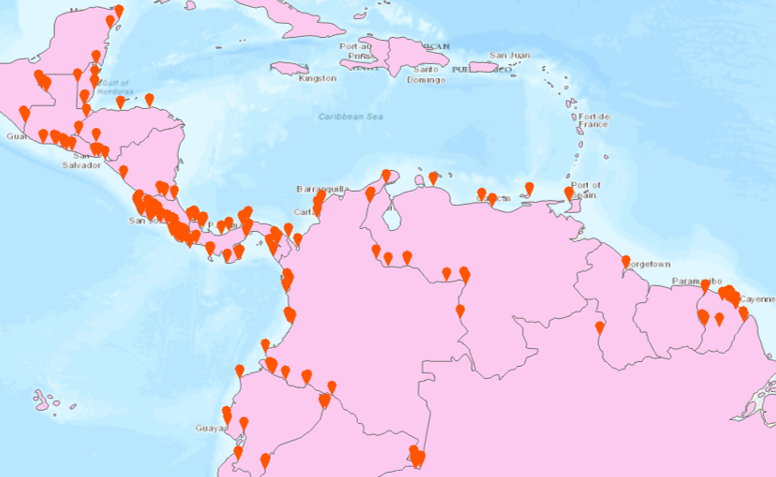
\includegraphics[width=0.8\linewidth]{./coun_cleanCoordinates} 

}

\caption{Fig 1. Scheme representing the main steps of the Locating KBAs workflow}\label{fig:gaps map 1}
\end{figure}

\begin{itemize}
\item
  \begin{enumerate}
  \def\labelenumi{\arabic{enumi}.}
  \setcounter{enumi}{3}
  \tightlist
  \item
    We will remove the coordinates assigned to zoos, botanical gardens,
    herbaria, universities and museums
  \end{enumerate}
\end{itemize}

\begin{Shaded}
\begin{Highlighting}[]
\NormalTok{data }\OtherTok{\textless{}{-}}\NormalTok{ flags }\SpecialCharTok{\%\textgreater{}\%}
  \FunctionTok{filter}\NormalTok{(.inst }\SpecialCharTok{==} \ConstantTok{TRUE}\NormalTok{) }\SpecialCharTok{\%\textgreater{}\%}
  \FunctionTok{droplevels}\NormalTok{()}
\end{Highlighting}
\end{Shaded}

\hypertarget{species-distributions}{%
\subsubsection{7. Species distributions}\label{species-distributions}}

Now we will remove the records that fall outside the species
distributions (with a \textasciitilde10 km buffer). For Colombia, we
will use the \href{http://biomodelos.humboldt.org.co/es}{Biomodelos
distributions}. For the species that had multiple hypothesis, we used
the distribution maps of Ayerbe, and for those that do not have a
Biomodelos distribution, we will use the IUCN distribution.

\emph{To see the code for merging the Biomodelos and IUCN distribution
refer to the ArcGIS Pro notebook called ``Biomodelos\_and\_IUCN''}

\hypertarget{biomodelos-and-iucn}{%
\paragraph{7.1. Biomodelos and IUCN}\label{biomodelos-and-iucn}}

\begin{Shaded}
\begin{Highlighting}[]
\CommentTok{\# Load the merged IUCN and biomodelos distributions for all sp}
\NormalTok{Bio\_IUCN }\OtherTok{\textless{}{-}} \FunctionTok{readOGR}\NormalTok{(}\StringTok{"F:/Connectivity/data/species\_distributions/Biomodelos\_and\_IUCN"}\NormalTok{, }\AttributeTok{layer =} \StringTok{"ALL\_sp"}\NormalTok{, }\AttributeTok{verbose =} \ConstantTok{TRUE}\NormalTok{)}
\end{Highlighting}
\end{Shaded}

\begin{verbatim}
## OGR data source with driver: ESRI Shapefile 
## Source: "F:\Connectivity\data\species_distributions\Biomodelos_and_IUCN", layer: "ALL_sp"
## with 92 features
## It has 3 fields
\end{verbatim}

\begin{Shaded}
\begin{Highlighting}[]
\CommentTok{\# Since the cc\_iucn requires to project the coordinates when applying a buffer, }
\CommentTok{\# we will upload the distributions with a geodesic buffer of 0.1° (\textasciitilde{} 10km) produced in ArcGIS Pro. }

\NormalTok{Bio\_IUCN\_buffer }\OtherTok{\textless{}{-}} \FunctionTok{readOGR}\NormalTok{(}\StringTok{"F:/Connectivity/data/species\_distributions/Biomodelos\_and\_IUCN"}\NormalTok{, }\AttributeTok{layer =} \StringTok{"ALL\_sp\_buffer"}\NormalTok{, }\AttributeTok{verbose =} \ConstantTok{TRUE}\NormalTok{)}
\end{Highlighting}
\end{Shaded}

\begin{verbatim}
## OGR data source with driver: ESRI Shapefile 
## Source: "F:\Connectivity\data\species_distributions\Biomodelos_and_IUCN", layer: "ALL_sp_buffer"
## with 18 features
## It has 3 fields
\end{verbatim}

\begin{Shaded}
\begin{Highlighting}[]
\CommentTok{\# Add a column named binomial to the ebird datase, since is the column that the }
\CommentTok{\# shapefile has }
\NormalTok{data\_Bio\_IUCN }\OtherTok{\textless{}{-}}\NormalTok{ data }\SpecialCharTok{\%\textgreater{}\%} 
  
  \FunctionTok{mutate}\NormalTok{(}\AttributeTok{BINOMIAL =} \StringTok{\textasciigrave{}}\AttributeTok{SCIENTIFIC NAME}\StringTok{\textasciigrave{}}\NormalTok{) }\SpecialCharTok{\%\textgreater{}\%}
  
  \CommentTok{\# Include only the species that had a unique Biomodelos distribution}
  \FunctionTok{filter}\NormalTok{(BINOMIAL }\SpecialCharTok{\%in\%} \FunctionTok{c}\NormalTok{(}\StringTok{"Ara macao"}\NormalTok{, }\StringTok{"Ara militaris"}\NormalTok{, }\StringTok{"Buteo albigula"}\NormalTok{, }\StringTok{"Campephilus pollens"}\NormalTok{, }\StringTok{"Crypturellus erythropus"}\NormalTok{, }\StringTok{"Crypturellus kerriae"}\NormalTok{,   }
 \StringTok{"Crypturellus soui"}\NormalTok{, }\StringTok{"Grallaria hypoleuca"}\NormalTok{, }\StringTok{"Grallaria nuchalis"}\NormalTok{,     }
\StringTok{"Henicorhina leucophrys"}\NormalTok{, }\StringTok{"Micrastur semitorquatus"}\NormalTok{, }\StringTok{"Mitu salvini"}\NormalTok{,            }
\StringTok{"Mitu tomentosum"}\NormalTok{, }\StringTok{"Phaethornis malaris"}\NormalTok{,  }\StringTok{"Picumnus lafresnayi"}\NormalTok{,    }
\StringTok{"Picumnus squamulatus"}\NormalTok{, }\StringTok{"Pyrrhura melanura"}\NormalTok{, }\StringTok{"Spizaetus ornatus"}\NormalTok{ )) }\SpecialCharTok{\%\textgreater{}\%}
  
  \FunctionTok{droplevels}\NormalTok{()}

\CommentTok{\# Remove records that fall outside the distribution with the 0.1° buffer }
\NormalTok{data\_Bio\_IUCN\_clean }\OtherTok{\textless{}{-}} \FunctionTok{cc\_iucn}\NormalTok{(}\AttributeTok{x =}\NormalTok{ data\_Bio\_IUCN, }
                \AttributeTok{range =}\NormalTok{ Bio\_IUCN\_buffer, }
                \AttributeTok{lon =} \StringTok{"LONGITUDE"}\NormalTok{, }
                \AttributeTok{lat =} \StringTok{"LATITUDE"}\NormalTok{,}
                \AttributeTok{species =} \StringTok{"BINOMIAL"}\NormalTok{,}
                \AttributeTok{verbose =} \ConstantTok{TRUE}\NormalTok{)}
\end{Highlighting}
\end{Shaded}

\begin{verbatim}
## Testing natural ranges
\end{verbatim}

\begin{verbatim}
## Removed 4663 records.
\end{verbatim}

\hypertarget{ayerbe-and-iucn}{%
\paragraph{7.2. Ayerbe and IUCN}\label{ayerbe-and-iucn}}

\begin{Shaded}
\begin{Highlighting}[]
\CommentTok{\# Load the merged IUCN and ayerbe distributions for all sp with a 0.1° buffer}

\NormalTok{Aye\_IUCN\_buffer }\OtherTok{\textless{}{-}} \FunctionTok{readOGR}\NormalTok{(}\StringTok{"F:/Connectivity/data/species\_distributions/Ayerbe\_and\_IUCN"}\NormalTok{, }\AttributeTok{layer =} \StringTok{"ALL\_sp\_buffer"}\NormalTok{, }\AttributeTok{verbose =} \ConstantTok{TRUE}\NormalTok{)}
\end{Highlighting}
\end{Shaded}

\begin{verbatim}
## OGR data source with driver: ESRI Shapefile 
## Source: "F:\Connectivity\data\species_distributions\Ayerbe_and_IUCN", layer: "ALL_sp_buffer"
## with 12 features
## It has 3 fields
\end{verbatim}

\begin{Shaded}
\begin{Highlighting}[]
\CommentTok{\# Add a column named binomial to the ebird datase, since is the column that the }
\CommentTok{\# shapefile has }
\NormalTok{data\_Aye\_IUCN }\OtherTok{\textless{}{-}}\NormalTok{ data }\SpecialCharTok{\%\textgreater{}\%} 
  
  \FunctionTok{mutate}\NormalTok{(}\AttributeTok{BINOMIAL =} \StringTok{\textasciigrave{}}\AttributeTok{SCIENTIFIC NAME}\StringTok{\textasciigrave{}}\NormalTok{) }\SpecialCharTok{\%\textgreater{}\%}
  
  \CommentTok{\# Include only the species that had multiple or non Biomodelos distribution and had an Ayerbe distribution}
  \FunctionTok{filter}\NormalTok{(BINOMIAL }\SpecialCharTok{\%in\%} \FunctionTok{c}\NormalTok{(}\StringTok{"Myioborus flavivertex"}\NormalTok{, }\StringTok{"Grallaria flavotincta"}\NormalTok{, }\StringTok{"Picumnus cinnamomeus"}\NormalTok{, }\StringTok{"Odontophorus hyperythrus"}\NormalTok{, }\StringTok{"Crypturellus berlepschi"}\NormalTok{, }\StringTok{"Tangara johannae"}\NormalTok{, }\StringTok{"Ramphastos brevis"}\NormalTok{, }\StringTok{"Spizaetus isidori"}\NormalTok{, }\StringTok{"Pseudastur albicollis"}\NormalTok{, }\StringTok{"Hypopyrrhus pyrohypogaster"}\NormalTok{, }\StringTok{"Patagioenas goodsoni"}\NormalTok{, }\StringTok{"Ognorhynchus icterotis"}\NormalTok{)) }\SpecialCharTok{\%\textgreater{}\%}
  
  \FunctionTok{droplevels}\NormalTok{()}

\CommentTok{\# Remove records that fall outside the distribution with the 0.1° buffer }
\NormalTok{data\_Aye\_IUCN\_clean }\OtherTok{\textless{}{-}} \FunctionTok{cc\_iucn}\NormalTok{(}\AttributeTok{x =}\NormalTok{ data\_Aye\_IUCN, }
                \AttributeTok{range =}\NormalTok{ Aye\_IUCN\_buffer, }
                \AttributeTok{lon =} \StringTok{"LONGITUDE"}\NormalTok{, }
                \AttributeTok{lat =} \StringTok{"LATITUDE"}\NormalTok{,}
                \AttributeTok{species =} \StringTok{"BINOMIAL"}\NormalTok{,}
                \AttributeTok{verbose =} \ConstantTok{TRUE}\NormalTok{)}
\end{Highlighting}
\end{Shaded}

\begin{verbatim}
## Testing natural ranges
\end{verbatim}

\begin{verbatim}
## Removed 3363 records.
\end{verbatim}

\hypertarget{only-iucn}{%
\paragraph{7.3. Only IUCN}\label{only-iucn}}

\begin{Shaded}
\begin{Highlighting}[]
\CommentTok{\# Only one species does not have a Biomodelos or Ayerbe distribution: Grallaria bangsi}

\CommentTok{\# Load the IUCN distribution with the 0.1° buffer}
\NormalTok{IUCN\_buffer }\OtherTok{\textless{}{-}} \FunctionTok{readOGR}\NormalTok{(}\StringTok{"F:/Connectivity/data/species\_distributions/IUCN"}\NormalTok{, }\AttributeTok{layer =} \StringTok{"Grallaria\_bangsi\_buffer"}\NormalTok{, }\AttributeTok{verbose =} \ConstantTok{TRUE}\NormalTok{)}
\end{Highlighting}
\end{Shaded}

\begin{verbatim}
## OGR data source with driver: ESRI Shapefile 
## Source: "F:\Connectivity\data\species_distributions\IUCN", layer: "Grallaria_bangsi_buffer"
## with 1 features
## It has 1 fields
\end{verbatim}

\begin{Shaded}
\begin{Highlighting}[]
\CommentTok{\# Add a column named binomial to the ebird datase, since is the column that the }
\CommentTok{\# shapefile has }
\NormalTok{data\_IUCN }\OtherTok{\textless{}{-}}\NormalTok{ data }\SpecialCharTok{\%\textgreater{}\%} 
  
  \FunctionTok{mutate}\NormalTok{(}\AttributeTok{BINOMIAL =} \StringTok{\textasciigrave{}}\AttributeTok{SCIENTIFIC NAME}\StringTok{\textasciigrave{}}\NormalTok{) }\SpecialCharTok{\%\textgreater{}\%}
  
  \CommentTok{\# Include only the species that had multiple or non Biomodelos distribution and had an Ayerbe distribution}
  \FunctionTok{filter}\NormalTok{(BINOMIAL }\SpecialCharTok{==} \StringTok{"Grallaria bangsi"}\NormalTok{) }\SpecialCharTok{\%\textgreater{}\%}
  
  \FunctionTok{droplevels}\NormalTok{()}

\CommentTok{\# Remove records that fall outside the distribution with the 0.1° buffer }
\NormalTok{data\_IUCN\_clean }\OtherTok{\textless{}{-}} \FunctionTok{cc\_iucn}\NormalTok{(}\AttributeTok{x =}\NormalTok{ data\_IUCN, }
                \AttributeTok{range =}\NormalTok{ IUCN\_buffer, }
                \AttributeTok{lon =} \StringTok{"LONGITUDE"}\NormalTok{, }
                \AttributeTok{lat =} \StringTok{"LATITUDE"}\NormalTok{,}
                \AttributeTok{species =} \StringTok{"BINOMIAL"}\NormalTok{,}
                \AttributeTok{verbose =} \ConstantTok{TRUE}\NormalTok{)}
\end{Highlighting}
\end{Shaded}

\begin{verbatim}
## Testing natural ranges
\end{verbatim}

\begin{verbatim}
## Removed 0 records.
\end{verbatim}

\hypertarget{bind-all-records}{%
\paragraph{7.4. Bind all records}\label{bind-all-records}}

Now, we will combine the three tables

\begin{Shaded}
\begin{Highlighting}[]
\NormalTok{data }\OtherTok{\textless{}{-}} \FunctionTok{rbind}\NormalTok{(data\_IUCN\_clean, data\_Aye\_IUCN\_clean, data\_Bio\_IUCN\_clean)}
\end{Highlighting}
\end{Shaded}

\begin{Shaded}
\begin{Highlighting}[]
\CommentTok{\# Create a year field }
\NormalTok{data }\OtherTok{\textless{}{-}}\NormalTok{ data }\SpecialCharTok{\%\textgreater{}\%} \FunctionTok{mutate}\NormalTok{(}\StringTok{"YEAR\_OBSERVATION"} \OtherTok{=} \FunctionTok{format}\NormalTok{(}\StringTok{\textasciigrave{}}\AttributeTok{OBSERVATION DATE}\StringTok{\textasciigrave{}}\NormalTok{, }\AttributeTok{format =} \StringTok{"\%Y"}\NormalTok{))}

\FunctionTok{write.csv}\NormalTok{(data, }\StringTok{"F:/Connectivity/outputs/01\_cleanOcurrences/cleanedData\_phase1.csv"}\NormalTok{, }\AttributeTok{row.names =} \ConstantTok{FALSE}\NormalTok{)}
\end{Highlighting}
\end{Shaded}

\hypertarget{divide-before-and-after-2000}{%
\section{8. Divide before and after
2000}\label{divide-before-and-after-2000}}

\begin{Shaded}
\begin{Highlighting}[]
\CommentTok{\# Calculate total number of records per species, and number of records before and after 2000}
\NormalTok{n\_total }\OtherTok{\textless{}{-}}\NormalTok{ data }\SpecialCharTok{\%\textgreater{}\%} \FunctionTok{group\_by}\NormalTok{(}\StringTok{\textasciigrave{}}\AttributeTok{SCIENTIFIC NAME}\StringTok{\textasciigrave{}}\NormalTok{) }\SpecialCharTok{\%\textgreater{}\%}\NormalTok{ dplyr}\SpecialCharTok{::}\FunctionTok{summarise}\NormalTok{(}\AttributeTok{n\_total =} \FunctionTok{n}\NormalTok{())}
\NormalTok{n\_2000 }\OtherTok{\textless{}{-}}\NormalTok{ data }\SpecialCharTok{\%\textgreater{}\%} \FunctionTok{filter}\NormalTok{(YEAR\_OBSERVATION }\SpecialCharTok{\textless{}=} \DecValTok{2000}\NormalTok{) }\SpecialCharTok{\%\textgreater{}\%} \FunctionTok{droplevels}\NormalTok{() }\SpecialCharTok{\%\textgreater{}\%} \FunctionTok{group\_by}\NormalTok{(}\StringTok{\textasciigrave{}}\AttributeTok{SCIENTIFIC NAME}\StringTok{\textasciigrave{}}\NormalTok{) }\SpecialCharTok{\%\textgreater{}\%} \FunctionTok{summarise}\NormalTok{(}\AttributeTok{n\_before\_2000 =} \FunctionTok{n}\NormalTok{())}
\NormalTok{n\_2021 }\OtherTok{\textless{}{-}}\NormalTok{ data }\SpecialCharTok{\%\textgreater{}\%} \FunctionTok{filter}\NormalTok{(YEAR\_OBSERVATION }\SpecialCharTok{\textgreater{}} \DecValTok{2000}\NormalTok{) }\SpecialCharTok{\%\textgreater{}\%} \FunctionTok{droplevels}\NormalTok{() }\SpecialCharTok{\%\textgreater{}\%} \FunctionTok{group\_by}\NormalTok{(}\StringTok{\textasciigrave{}}\AttributeTok{SCIENTIFIC NAME}\StringTok{\textasciigrave{}}\NormalTok{) }\SpecialCharTok{\%\textgreater{}\%} \FunctionTok{summarise}\NormalTok{(}\AttributeTok{n\_after\_2000 =} \FunctionTok{n}\NormalTok{())}

\NormalTok{n\_species }\OtherTok{\textless{}{-}} \FunctionTok{full\_join}\NormalTok{(n\_total, n\_2021, }\AttributeTok{by =} \StringTok{"SCIENTIFIC NAME"}\NormalTok{) }\SpecialCharTok{\%\textgreater{}\%} \FunctionTok{full\_join}\NormalTok{(n\_2000, }\AttributeTok{by =} \StringTok{"SCIENTIFIC NAME"}\NormalTok{) }

\FunctionTok{write.csv}\NormalTok{(n\_species, }\StringTok{"F:/Connectivity/outputs/01\_cleanOcurrences/cleanedData\_numberRecords\_phase1.csv"}\NormalTok{, }\AttributeTok{row.names =} \ConstantTok{FALSE}\NormalTok{)}
\end{Highlighting}
\end{Shaded}


\end{document}
